\documentclass{beamer}

% Theme and Custom Colors
\usetheme{CambridgeUS}
\definecolor{customblue}{RGB}{0, 119, 200}
\setbeamercolor{frametitle}{fg=customblue}
\setbeamercolor{title}{fg=customblue}
\setbeamercolor{itemize item}{fg=customblue}
\setbeamercolor{block title}{bg=customblue, fg=white}
\setbeamercolor{structure}{fg=customblue}
\setbeamercolor{progress bar in head/foot}{fg=customblue, bg=customblue}
\setbeamercolor{author in head/foot}{fg=white, bg=customblue}
\setbeamercolor{title in head/foot}{fg=customblue, bg=white} % done
\setbeamercolor{date in head/foot}{fg=customblue} % done
\setbeamercolor{section in head/foot}{bg=customblue, fg=white} %done
\setbeamercolor{headline}{bg=customblue, fg=white}

% Packages
\usepackage{graphicx}
\usepackage{amsmath}
\usepackage{hyperref}
\usepackage[font=scriptsize]{caption}


% Title Page Information
\title{Beam and Ball Controller Design}
\subtitle{Simulating and Controlling a Ball-and-Beam System \\Using State Feedback Controller}
\author{Alexander Brown}
\date{December 2, 2024}
\institute{EE486 - Final Project}

\begin{document}

% Title Slide
\begin{frame}
    \titlepage
\end{frame}

\begin{frame}{Project Overview}
    \textbf{Problem Statement:} 
    The ball-and-beam system is inherently unstable, requiring a controller to manage coupled dynamics, stabilize the system, and minimize error and control effort.

    \vspace{0.5cm}
    \textbf{Objective:} 
    \begin{itemize} 
        \item Design \& implement feedback controller for a ball-and-beam system.
	\begin{itemize}
		\item Adjust the beam angle to return the ball to center position.
	\end{itemize}
        \item Simulate the system using a 3D model in Simscape Multibody.
    \end {itemize}

    \vspace{0.5cm}
    \textbf{Technical Approach:}
    \begin{itemize}
        \item Derive system dynamics using Newtonian and Lagrangian methods.
        \item Linearize nonlinear dynamics for control design.
        \item Use state-space methods to design and implement feedback control.
    \end{itemize}
\end{frame}

% slide 2
\begin{frame}{Challenges and Control Goals}
        \textbf{\small System Challenges:}
        \begin{itemize}
	    \small
            \item Amplifies small angular changes into large ball displacements.
            \item Coupled ball and beam dynamics complicate control.
        \end{itemize}

        \textbf{\small Control Goals:}
        \begin{itemize}
	    \small
            \item Stabilize the ball at the beam's center position.
            \item Minimize overshoot, settling time, and steady-state error.
        \end{itemize}
        
        \centering
	\begin{figure}
	        \fbox{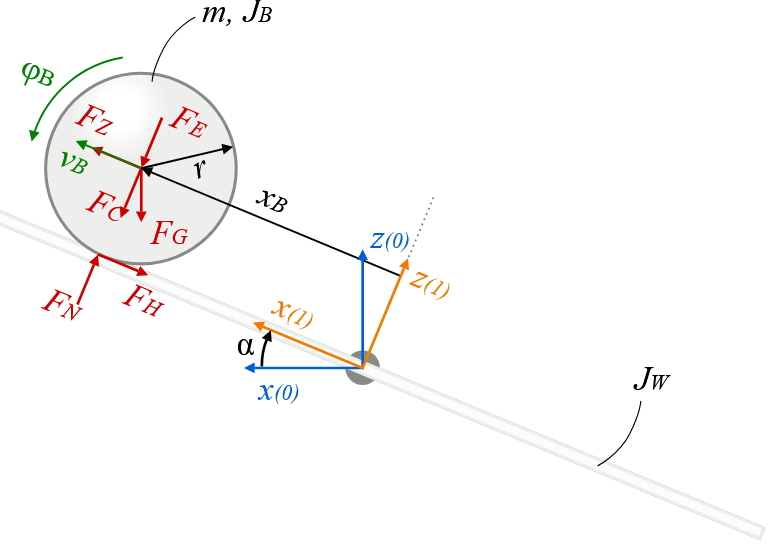
\includegraphics[width=0.45\textwidth]{Figures/system_diag_wiki_left.png}}  % Adds a box around the image
	        \caption{Ball-and-Beam Dynamics. \tiny Source: \href{https://en.wikipedia.org/wiki/Ball_and_beam}{Wikipedia}}
	        \label{fig:ball_and_beam}
    	\end{figure}
\end{frame}

% slide 3
\begin{frame}{Degrees of Freedom and Modeling Approach}
    \textbf{Degrees of Freedom:}
    \begin{itemize}
        \item Ball position (\(x\)) along the beam axis.
        \item Beam angle (\(\theta\)) relative to the horizontal.
    \end{itemize}

    \vspace{0.2cm}
    \textbf{Modeling Approach:}
    \begin{itemize}
        \item Newtonian Mechanics used to derive equations of motion:
        \begin{itemize}
            \item \textbf{\(\boldsymbol{F = ma}\):} Describes the translational motion of the ball.
            \item \textbf{\(\boldsymbol{\tau = I \alpha}\):} Describes the rotational motion of the beam.
        \end{itemize}
        
        \item Lagrangian Mechanics used to formulate system dynamics:
        \begin{itemize}
            \item \textbf{Kinetic Energy (\(T\)):} The energy due to motion.
            \item \textbf{Potential Energy (\(V\)):} The energy due to the ball’s position in a gravitational field.
        \end{itemize}
    \end{itemize}
\end{frame}


% slide 4
\begin{frame}{System Parameters and State-Space Representation}
    \textbf{\small Assumed Parameters:}
    \begin{itemize}
        \small
        \item \small Beam:
        \begin{itemize}
            \footnotesize
            \item Length: \(L = 1.0\ \mathrm{m}\)
            \item Width: \(w = 0.05\ \mathrm{m}\)
            \item Height: \(h = 0.1\ \mathrm{m}\)
        \end{itemize}
        \item \small Ball:
        \begin{itemize}
            \footnotesize
            \item Mass: \(m = 0.5\ \mathrm{kg}\)
            \item Radius: \(r = 0.05\ \mathrm{m}\)
            \item Moment of inertia: \(I = 0.02\ \mathrm{kg{\cdot}m^2}\)
        \end{itemize}
        \item \small Gravitational acceleration: \(g = 9.81\ \mathrm{m/s^2}\)
    \end{itemize}

    \vspace{0.2cm}
    \textbf{\small State-Space Representation:}
    \begin{itemize}
        \footnotesize
        \item Expressed as \(\dot{x} = A x + B u, \quad y = C x + D u\).
        \item System matrices:
        \[
        A = \begin{bmatrix} 
        0 & 1 & 0 & 0 \\
        0 & 0 & \frac{g}{L} & 0 \\
        0 & 0 & 0 & 1 \\
        0 & 0 & -\frac{m g r}{I} & 0 
        \end{bmatrix}, \quad 
        B = \begin{bmatrix} 
        0 \\ 
        0 \\ 
        0 \\ 
        \frac{1}{I} 
        \end{bmatrix}.
        \]
    \end{itemize}
\end{frame}

% slide 5
\begin{frame}{Controller Design}
    \small
    \textbf{Objective:} Minimize the cost function to balance performance and control effort:
    \[
    J = \int_0^\infty \left( x^T Q x + u^T R u \right) dt
    \]

    \textbf{Design Parameters:}
    \begin{itemize}
        \item \(\texttt{Q = diag([200, 10, 10, 10])}\): Penalizes state deviations.
        \begin{itemize}
            \footnotesize
            \item Prioritizes ball position (\(x\)) and beam angle (\(\theta\)).
        \end{itemize}
        \item \(\texttt{R = 1}\): Penalizes excessive control effort.
    \end{itemize}

    \textbf{Result:} The feedback gain \(K\) is computed in MATLAB using:
    \begin{center}
        \texttt{K = lqr(A, B, Q, R);}
    \end{center}

    \textbf{Control Law:} The control law uses \(K\) to stabilize the ball-and-beam system and minimize deviations in state variables. The control input is calculated as
    \[
    u = -Kx.
    \]
\end{frame}

% slide 6
\begin{frame}{MATLAB Integration}
    \textbf{Purpose:} Use MATLAB for controller design and performance evaluation.

    \vspace{0.3cm}
    \textbf{MATLAB Script Features:}
    \begin{itemize}
        \item Defines system parameters and state-space matrices.
        \item Controller Design.
        \item Performance Metrics:
        \begin{itemize}
            \footnotesize
            \item \textbf{IAE:} Measures overall error magnitude for control precision.
            \item \textbf{ISE:} Emphasizes large errors for stability assessment.
            \item \textbf{ITAE:} Penalizes sustained errors for improved settling time.
            \item Overshoot and settling time: Assess transient response behavior.
        \end{itemize}
    \end{itemize}

    \vspace{0.3cm}
    \textbf{Output:} Plots system states (ball position, beam angle) and control effort over time.
\end{frame}

% slide 7
\begin{frame}{Simulation Results}
    \textbf{State Trajectories and Control Input:}
    \begin{itemize}
        \item Ball position (\(x\)) and beam angle (\(\theta\)) stabilize within 5 seconds.
        \item Control input (\(u\)) is smooth and free of oscillations, ensuring stability.
    \end{itemize}
    \begin{minipage}[t]{0.48\textwidth}
        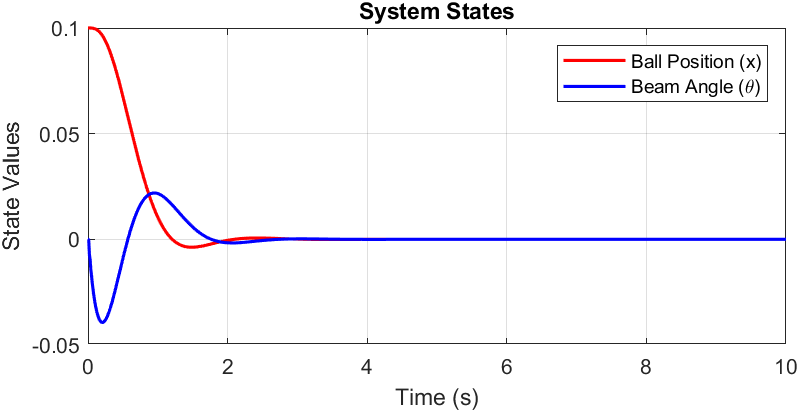
\includegraphics[width=\textwidth]{Figures/state_sim.png}
    \end{minipage}
    \hfill
    \begin{minipage}[t]{0.48\textwidth}
        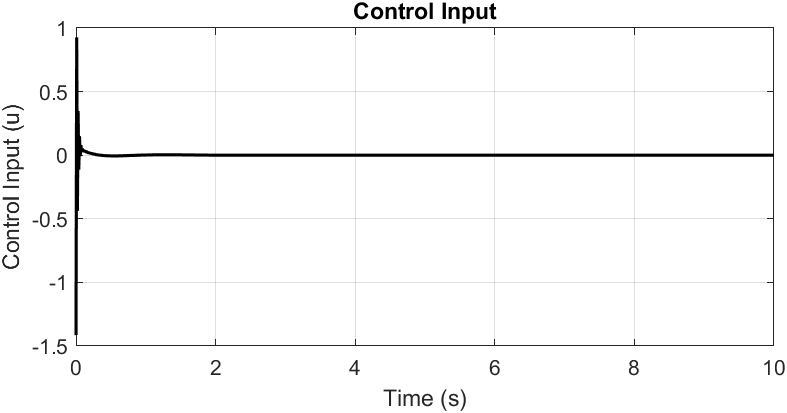
\includegraphics[width=\textwidth]{Figures/control_input_sim.png}
    \end{minipage}
    \textbf{Performance Metrics:}
    \begin{itemize}
        \item Integral Absolute Error (\(\text{IAE}\)): 0.06657.
        \item Integral Square Error (\(\text{ISE}\)): 0.00494.
        \item Integral Time-weighted Absolute Error (\(\text{ITAE}\)): 0.02813.
    \end{itemize}
\end{frame}

\begin{frame}{Simulink System Diagram}
    \textbf{Purpose:} Simulate real-world dynamics of the ball-and-beam system using MATLAB's Simscape library.

    \vspace{0.3cm}
    \textbf{Key Features:}
    \begin{itemize}
        \small
        \item Models system dynamics with realistic physics (ball and beam motion).
        \item Includes key components:
        \begin{itemize}
            \footnotesize
            \item System Dynamics: Ball and beam subsystems.
            \item Integral Compensation: Corrects steady-state errors.
            \item LQR Controller: Stabilizes the system.
        \end{itemize}
    \end{itemize}

    \vspace{0.3cm}
    \centering
    \begin{figure}
        \fbox{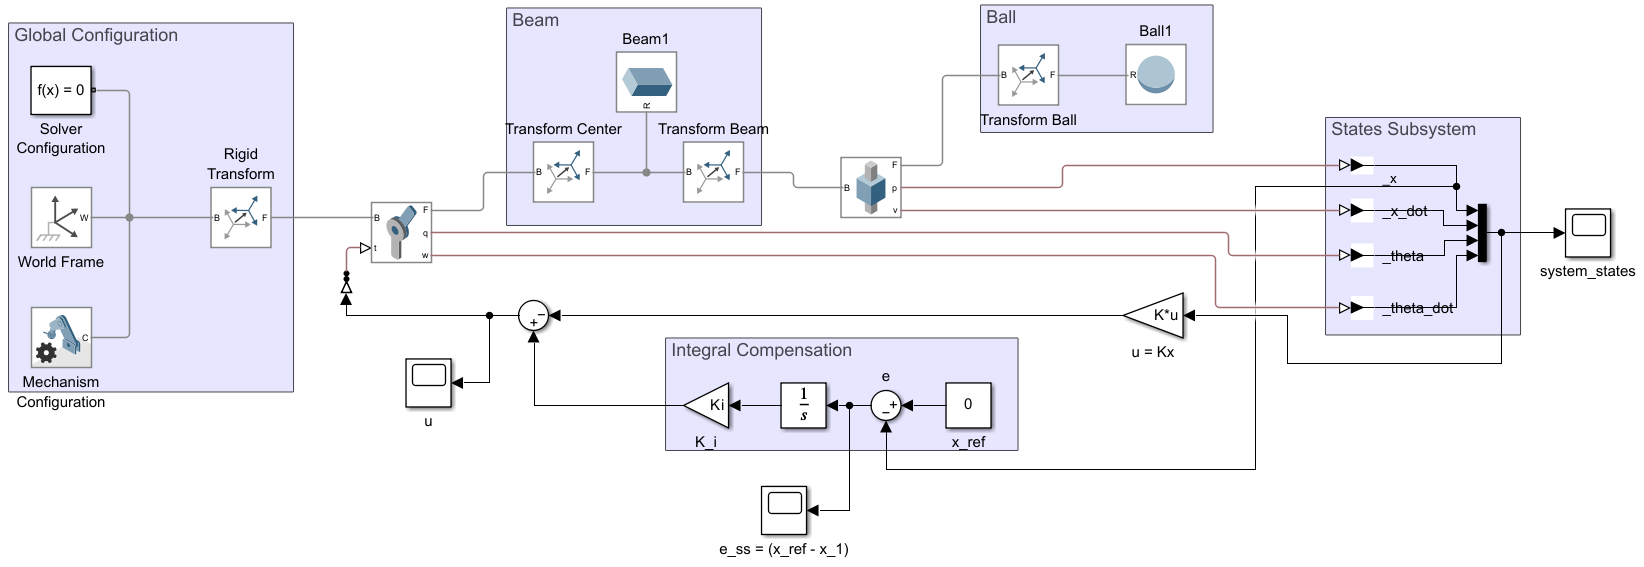
\includegraphics[width=0.95\textwidth]{Figures/simulink_model.png}}
        \caption{\footnotesize Simulink model for ball-and-beam dynamics.}
        \label{fig:simulink_model}
    \end{figure}
\end{frame}

% Slide for 3D Model Simulation Results
\begin{frame}{3D Model Simulation Results}
    \centering
    \begin{columns}[T] % Align columns at the top
        \begin{column}{0.48\textwidth}
            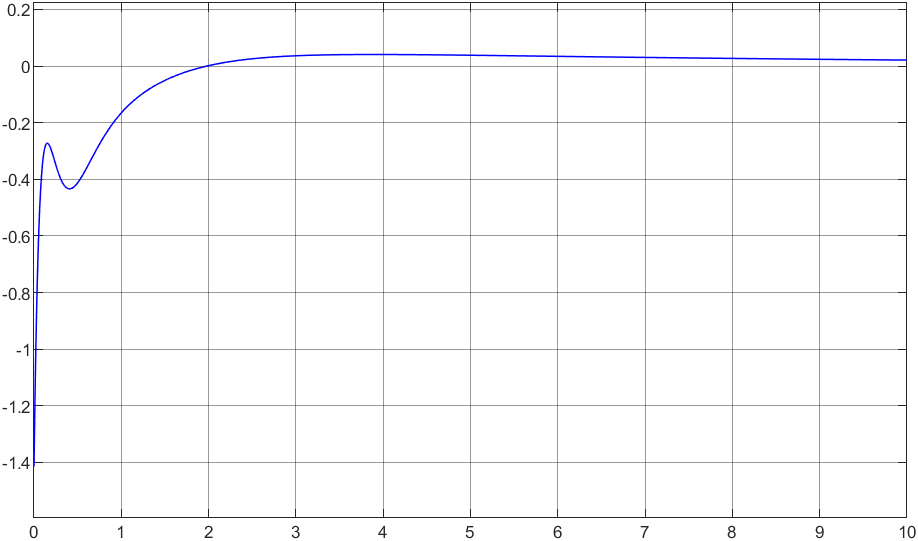
\includegraphics[width=0.9\textwidth]{Figures/control_input_scope.png}
	    \captionof{figure}{Control input - simulation scope.}
        \end{column}
        \begin{column}{0.48\textwidth}
            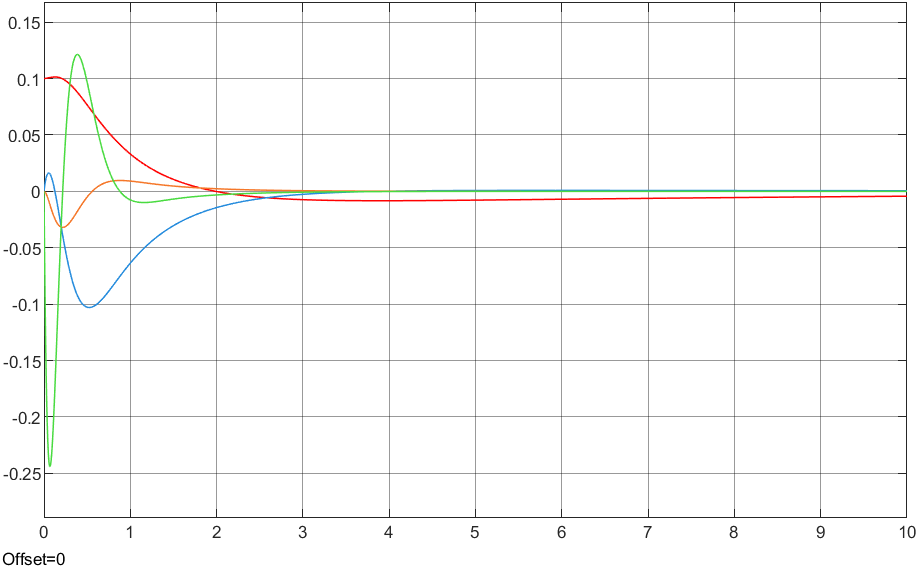
\includegraphics[width=0.85\textwidth]{Figures/states_scope.png}
	    \captionof{figure}{State trajectories -  simulation scope.}
	    \begin{itemize}
		\tiny
                \item \textcolor{red}{Red:} \(x\) (Ball position)
                \item \textcolor{blue}{Blue:} \(\dot{x}\) (Ball velocity)
                \item \textcolor{orange}{Orange:} \(\theta\) (Beam angle)
                \item \textcolor{green}{Green:} \(\dot{\theta}\) (Beam angular velocity)
            \end{itemize}
        \end{column}
    \end{columns}
    \begin{flushleft}
    \textbf{\small Insights:}
    \begin{itemize}
	\footnotesize
        \item The system stabilizes within 5 seconds with minimal oscillations.
        \item The control input indicates energy efficiency.
    \end{itemize}
	\end{flushleft}
\end{frame}




% slide 9
\begin{frame}{Challenges and Future Work}
    \textbf{Challenges:}
    \begin{itemize}
        \item Sensitivity to parameter changes: ball mass (\(m\)) and beam length (\(L\)).
        \item Limitations of linearization for large beam angles (\(\theta\)).
        \item Initial controller design using pole placement was ineffective:
        \begin{itemize}
            \footnotesize
            \item Resulted in excessive oscillations, reducing stability.
            \item Required high control input, impractical for physical systems.
            \item LQR was chosen for its ability to balance control effort and system stability.
        \end{itemize}
    \end{itemize}

    \vspace{0.2cm}
    \textbf{Potential Improvements:}
    \begin{itemize}
        \item Model external disturbances (e.g., friction) to test system robustness.
        \item Integrate filtering for noise reduction and state estimation.
        \item Develop dynamic reference tracking for moving target positions.
        \item Investigate nonlinear control strategies for large-angle behaviors.
    \end{itemize}
\end{frame}

% Slide 10
\begin{frame}{Conclusion}
    \textbf{Key Achievements:}
    \begin{itemize}
        \item Successfully modeled the ball-and-beam system dynamics using Newtonian and Lagrangian mechanics.
        \item Designed an LQR controller to stabilize the system, achieving:
        \begin{itemize}
            \footnotesize
            \item Minimal overshoot and short settling time.
            \item Smooth and stable control input (\(u\)).
        \end{itemize}
        \item Validated the system through MATLAB analysis and Simulink simulations.
    \end{itemize}

    \vspace{0.2cm}
    \textbf{Outcomes:}
    \begin{itemize}
        \item Visualized results through 2D plots and 3D animations, providing insights into system performance.
        \item Identified limitations (e.g., sensitivity to parameter variations, large-angle behaviors) for future exploration.
    \end{itemize}
\end{frame}

% Final Slide
\begin{frame}
    \centering
    \vspace{1.5cm}
    \Huge{\textbf{Thank You}}
    
    \vspace{0.5cm}
    \Large
    \textit{Questions or Comments?}
    
    \vspace{1.5cm}
    \normalsize
    \textbf{Contact Information:} \\
    Alexander Brown \\
    \href{mailto:ajb0083@uah.edu}{ajb0083@uah.edu} \\
    EE486 - Final Project
\end{frame}


\end{document}
